\chapter{Query Overview, Results and Evaluation}\label{results}
To analyse the functionality of the database systems, I devised a number of queries with ranging difficulties. The aim of the queries was to establish the limitations of the systems, and to discover the efficacy of the systems. A further objective was to identify any extra features the solutions provide which may be useful. For example any visualisations of graphical analysis which may enhance the exploration of the data. Chapter \ref{evaluationstrategy} provides a detailed explanation of the reasoning behind the queries. This chapter discusses the output and results of running the queries in the various query languages. This chapter also gives insight into the difficulty of writing the query, the usefulness of the output, the time taken for the query to run and any challenges I faced when throughout the process. Additionally included in this chapter is a general discussion which summarises the capabilities of the systems and aims to provide one with an understanding of the limitations of each of the systems (section  \ref{queryevaluation}).

\section{Query Overview}\label{output}
The screen captures, tables, graphs and charts illustrated in this chapter are based on the results of running the competency based queries on each database system. Table \ref{tab:competency} details each of the devised queries in English, provides a short description of the data expected to be returned and includes a rating characterisation. The rating characterisation ranges from 1 to 5, and while there is no science behind the rating it is to be used as a guide to aid the reader into understanding \textbf{1.} General complexity of the query. \textbf{2.} Fruitfulness of the data returned. \textbf{3.} Level of expectancy that the system will be able to accomplish the query (on a scale of 1 expected, to 5 unexpected).

The order in which I wrote, run and evaluated the queries reflects the complexity of the query itself. I started by implementing simple queries which one would expect each of the systems to successfully achieve. The difficulty of each query increased every time. The end point of this evaluation was when I had written a number of complex queries which would be used to assess the EMAGE dataset in real life scenarios. For example, query number 7 in table \ref{tab:competency} ``Calculate transitive closure''. Finding the hierarchical path of a structure is something which researchers and scientists are often trying to achieve when analysing an anatomy. For example in terms of a human anatomy, the finger is part of the hand which is joined to the wrist which is part of the arm which is joined to the shoulder and so forth. Therefore its inclusion in this examination was necessary. A full description of this query, its origins and output is provided below. 

\begin{table}[H]
\centering
\resizebox{\textwidth}{!}{
\begin{tabular}{|c|l|l|c|}
\hline
\textbf{Query Number} & \multicolumn{1}{c|}{\textbf{English}} & \multicolumn{1}{c|}{\textbf{Expected return}} & \textbf{Rating} \\ \hline
1 & All structures at Theiler Stage X. & Theiler Stage and Structure ID. & 1 \\ \hline
2 & \begin{tabular}[c]{@{}l@{}}All structures between Theiler\\ Stage X and Y.\end{tabular} & \begin{tabular}[c]{@{}l@{}}Structure ID, Theiler Stage X and Theiler Stage\\Y.\end{tabular} & 1 \\ \hline
3 & Where is Gene X expressed? & \begin{tabular}[c]{@{}l@{}}Name of the gene, the structure where the\\ gene was found and the EMAGE ID where the\\ gene was found.\end{tabular} & 2 \\ \hline
4 & What is expressed in structure X? & \begin{tabular}[c]{@{}l@{}}Name of the gene(s) found in the structure. The\\structure ID and the name of the structure.\\ The Theiler Stage(s) of the structure. The\\EMAGE ID of the structure.\end{tabular} & 3 \\ \hline
5 & \begin{tabular}[c]{@{}l@{}}Which genes are stored in\\ structures X and Y?\end{tabular} & \begin{tabular}[c]{@{}l@{}}Name and ID of the gene(s). The ID of\\structure X and ID of structure Y.\end{tabular} & 4 \\ \hline
6 & \begin{tabular}[c]{@{}l@{}}Which Genes are most\\ commonly co-expressed?\end{tabular} & \begin{tabular}[c]{@{}l@{}}Name of the gene(s) and the count of unique\\ structures the gene is expressed in.\end{tabular} & 5 \\ \hline
7 & Calculate transitive closure. & The name of each structure and its parent. & 5 \\ \hline
\end{tabular}}
\caption{Competency queries for each database system.}
\label{tab:competency}
\end{table}

There are a number of queries one could write which would output potentially interesting results and provide an alternative view of the data. However, the purpose of this examination was to evaluate the functionality of the solutions, assess the limitations of each of the systems and identify any interesting additional features. Thus there was no requirement to include these additional queries which would fail to affect the outcome of the examination.

\section{Query Results}\label{queryresults}
The following subsections provide the results of running the queries outlined in table \ref{tab:competency}. Included in the subsections is the statement written for every system for each of the queries, where I was able to achieve the intended outcome. I have also included the physical output for the first 3 queries. This is to provide the reader with an insight into what is returned from each database solution when running a query. I have only included the output for the first 3 queries as I felt that doing the same process for each query did not add any value to the examination.

At the end of each subsection is a short review of each query, intended to summarise the findings. Section \ref{queryevaluation} provides an in-depth evaluation of the query examination stage of the project as a whole, and compares and contrasts each solution.

\subsection*{Query 1 - All structures at Theiler Stage X}\label{query1}
The first query which I wrote for each of the databases aimed to retrieve the anatomy structure information at a given Theiler Stage. For the basis of these tests I hard coded the Theiler stage; Theiler Stage 4 in this instance.  The minimum amount of data expected to be returned from this query is the structure ID, structure name and Theiler Stage. This query is not complex and one would expect that each database will possess the required functionality to handle this query and return the expected output.

\subsubsection*{MySQL - Query 1 statement}\label{mysqlquery1statement}
The MySQL query shown in code snippet \ref{code:mysqlquery1} successfully returned the expected output. The query was straightforward and only required a single join of the Stages and Anatomy Structures table. I was able to use the ``AS'' keyword to manually define an alias for the column headings of the returned data. The use of this keyword enhances the clarity of the output and allows one to easily identify the data being represented, as illustrated in figure \ref{fig:mysqlquery1}. Without the inclusion of the ``AS'' keyword, the headings of the returned data would be the same as the column names in the select statement. For example, ``StructureID'' would be ``AnatomyStructures.accession'' and ``StructureName'' would be ``AnatomyStructures.term''. The official MySQL documentation suggests It is good practice to explicitly use the ``AS'' keyword for all column names \cite{mysqlselectwebsite}.

\begin{lstlisting}[language=SQL, caption=MySQL Query 1 statement. All structures at Theiler Stage 4, label=code:mysqlquery1]
SELECT t1.accession AS StructureID, t1.term AS StructureName, t2.theilerstage AS TheilerStage, t2.dpc AS DPC
FROM AnatomyStructures AS t1
INNER JOIN Stages AS t2
ON t1.stage_id = t2.id
WHERE t2.theilerstage = 4
ORDER BY 1
\end{lstlisting}

\subsubsection*{MySQL - Query 1 output}\label{mysqlquery1output}
Figure \ref{fig:mysqlquery1} is a screen capture of the resulting output from running the MySQL query in the command-line interface. As you can see it returns the data in a table format separated by dashed lines. The number of rows returned and time taken for the query to process is also included below the table.

The output for this query is clear and coherent. However, for this query there is only 4 columns of data being returned. The MySQL command-line tool is run in a machine terminal. The size of the terminal window is at maximum the size of the machines monitor. Thus it is often the case that when returning a large number of columns, the data can become scrambled and illegible.
\begin{figure}[H]\begin{center}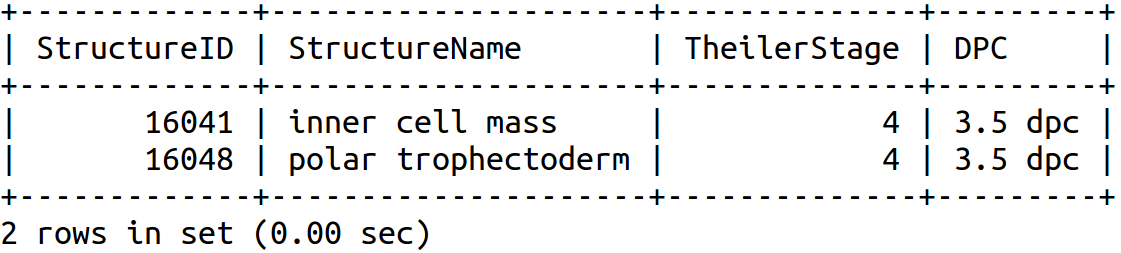
\includegraphics[height=4cm,width=0.9\linewidth]{images/mysqlquery1}\caption{MySQL command-line tool output - Query 1}\label{fig:mysqlquery1}\end{center}\end{figure}
One way to avoid this is to change the zoom level of the terminal. Depending on the volume of data returned, this can have little to no affect as the further out one zooms, the smaller the font becomes. This can often be a hindrance of using the MySQL command-line tool for advanced queering of large, multicolumn datasets.

\subsubsection*{MongoDB - Query 1 statement}\label{mongoquery1statement}
The MongoDB query shown in code snippet \ref{code:mongoquery1} successfully returned the expected output. The query is much shorter than that of the MySQL query but returns the same data.

\begin{lstlisting}[language=json, caption=MongoDB Query 1 statement. All structures at Theiler Stage 4, label=code:mongoquery1]
db.emage.find({
    "stage.theilerstage":4
    },
    {
    "_id" : 0,
    "stage.theilerstage" : 1,
    "stage.dpc" : 1,
    "textannotation.anatomystructure.structureID" : 1,
    "textannotation.anatomystructure.term" : 1
     }).pretty();
\end{lstlisting}

\subsubsection*{MongoDB - Query 1 output}\label{mongoquery1output}

\begin{figure}[H]\begin{center}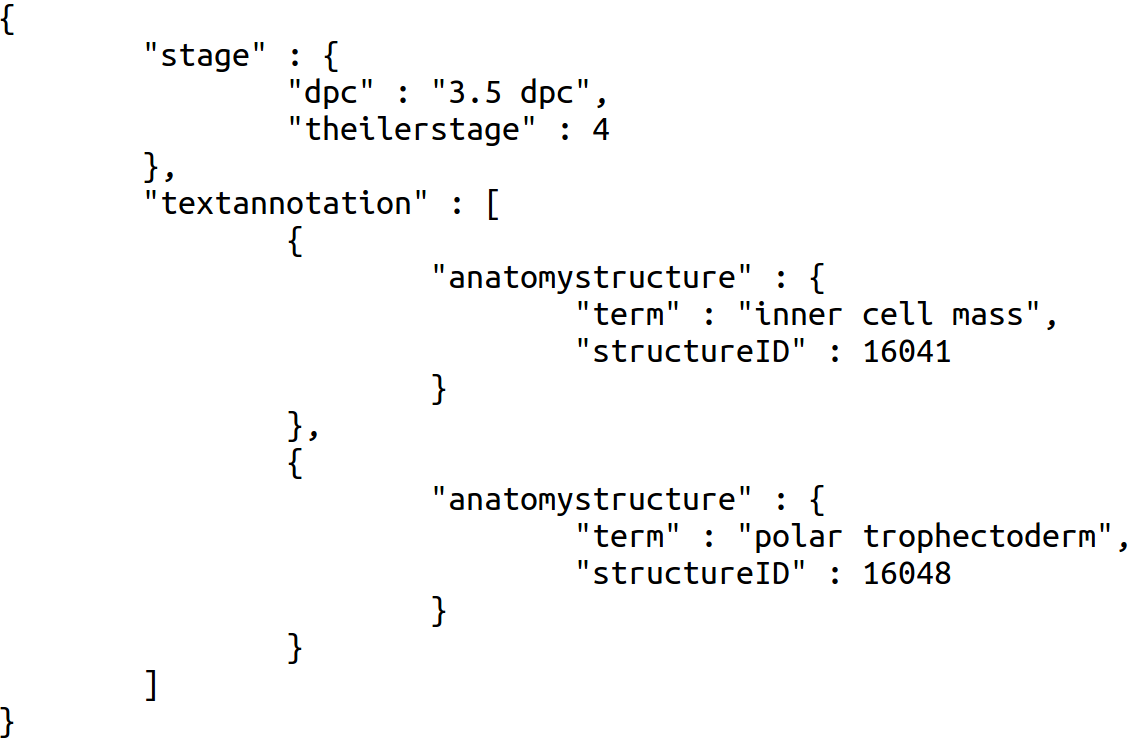
\includegraphics[width=1\linewidth]{images/mongoquery1}\caption{MongoDB command-line tool output - Query 1}\label{fig:mongoquery1}\end{center}\end{figure}

\subsubsection*{Neo4j - Query 1 statement}\label{neoquery1statement}

\begin{lstlisting}[language=SQL, caption=Neo4j Query 1 statement. All structures at Theiler Stage 4, label=code:neoquery1]
MATCH (struct:AnatomyStructure)-[r]->(stage:Stage)
WHERE stage.theilerStage = 4
RETURN struct, r, stage;
\end{lstlisting}

\subsubsection*{Neo4j - Query 1 output}\label{neoquery1output}

\begin{figure}[H]\begin{center}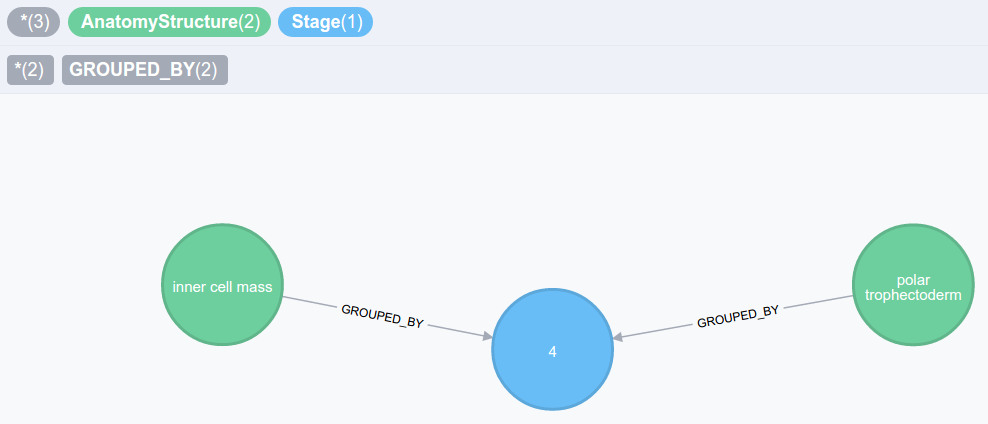
\includegraphics[width=1\linewidth]{images/neo4jquery1graph}\caption{Neo4j query 1 - All structures at Theiler Stage X}\label{fig:neo4jquery1graph}\end{center}\end{figure}

\begin{figure}[H]\begin{center}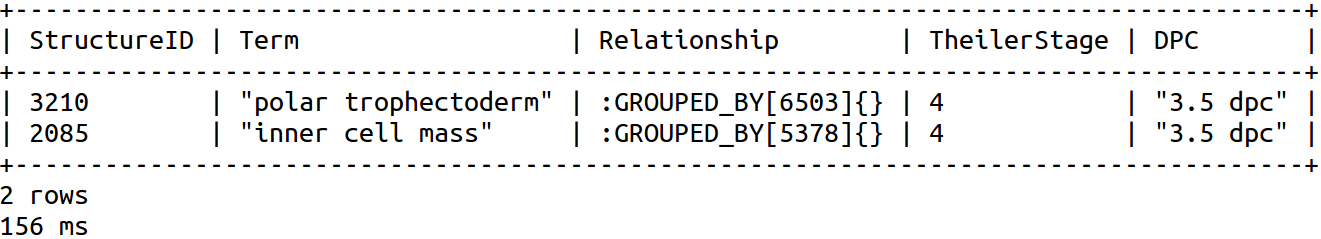
\includegraphics[height=4cm,width=0.9\linewidth]{images/neo4jquery1terminal}\caption{Neo4j query 1 - All structures at Theiler Stage X}\label{fig:neo4jquery1terminal}\end{center}\end{figure}

\subsubsection*{Apache Cassandra - Query 1 statement}\label{cassquery1statement}

\begin{lstlisting}[language=SQL, caption=, label=code:cassquery1]
SELECT *
FROM structurebystage
WHERE theilerstage = 4
AND detected = true;
\end{lstlisting}

\subsubsection*{Apache Cassandra - Query 1 output}\label{cassquery1output}

\begin{figure}[H]\begin{center}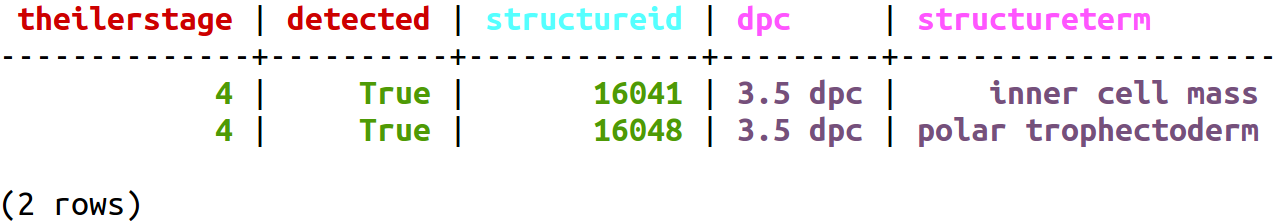
\includegraphics[height=4cm,width=0.9\linewidth]{images/cassandraquery1}\caption{Cassandra query 1 - All structures at Theiler Stage X}\label{fig:cassandraquery1}\end{center}\end{figure}

\subsection*{Query 1 - Review}\label{query1review}

\newpage
\subsection*{Query 2 - All structures between Theiler Stage X and Y}\label{query2}
The following code snippets represent the queries written for competency question 2.

\begin{itemize}[leftmargin=*]
\item \textbf{MySQL}
\end{itemize}

\begin{lstlisting}[language=SQL, caption=, label=code:mysqlquery2]
SELECT t1.accession, t2.theilerstage
FROM AnatomyStructures AS t1
INNER JOIN Stages AS t2
ON t1.stage_id = t2.id
INNER JOIN TextAnnotations AS t3
ON t1.id = t3.structure_id
WHERE t2.theilerstage BETWEEN 4 AND 7
AND t3.detected = 1
GROUP BY 1;
\end{lstlisting}

\begin{figure}[H]\begin{center}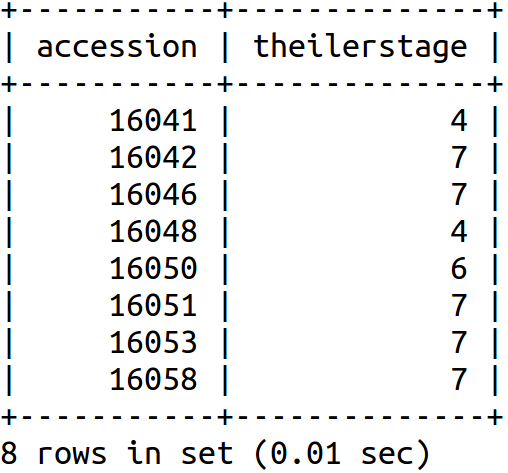
\includegraphics[height=7cm,width=0.4\linewidth]{images/mysqlquery2}\caption{MySQL query 2 - All structures between Theiler Stage X and Y}\label{fig:mysqlquery2}\end{center}\end{figure}

\begin{itemize}[leftmargin=*]
\item \textbf{MongoDB}
\end{itemize}

\begin{lstlisting}[language=json, caption=, label=code:mongoquery2]
db.emage.find({$and: [ {"textannotation.detected" : "True"},{ "stage.theilerstage": {$gte : 4 }},{ "stage.theilerstage": {$lte : 7 }}, {"textannotation.strength" : "detected"}]},{"textannotation.anatomystructure.structureID" : 1, "stage.theilerstage" : 1, "_id" : 0}).pretty();
\end{lstlisting}

\begin{itemize}[leftmargin=*]
\item \textbf{Neo4j}
\end{itemize}

\begin{lstlisting}[language=SQL, caption=, label=code:neoquery2]
MATCH (textannotation:TextAnnotation)-[]->(struct:AnatomyStructure)-[]->(stage:Stage)
WHERE stage.theilerStage >= 4 AND stage.theilerStage <=7 AND textannotation.detected = 1
RETURN struct.accession AS Accession, stage.theilerStage AS TheilerStage;
\end{lstlisting}

\begin{figure}[H]\begin{center}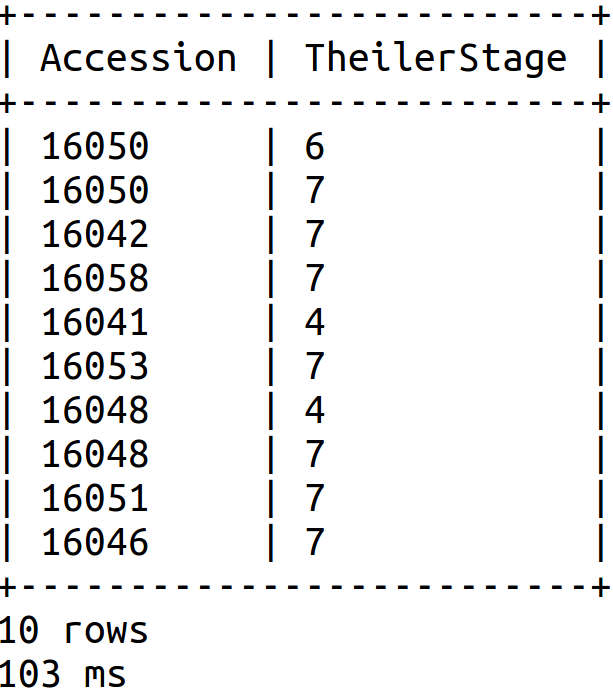
\includegraphics[height=7cm,width=0.4\linewidth]{images/neo4jquery2terminal}\caption{Neo4j query 2 - All structures between Theiler Stage X and Y}\label{fig:neo4jquery2terminal}\end{center}\end{figure}

\begin{itemize}[leftmargin=*]
\item \textbf{Cassandra}
\end{itemize}

\begin{lstlisting}[language=SQL, caption=, label=code:cassquery2]
SELECT *
FROM structurebystage
WHERE theilerstage IN (4,5,6,7)
AND detected = true;
\end{lstlisting}

\begin{figure}[H]\begin{center}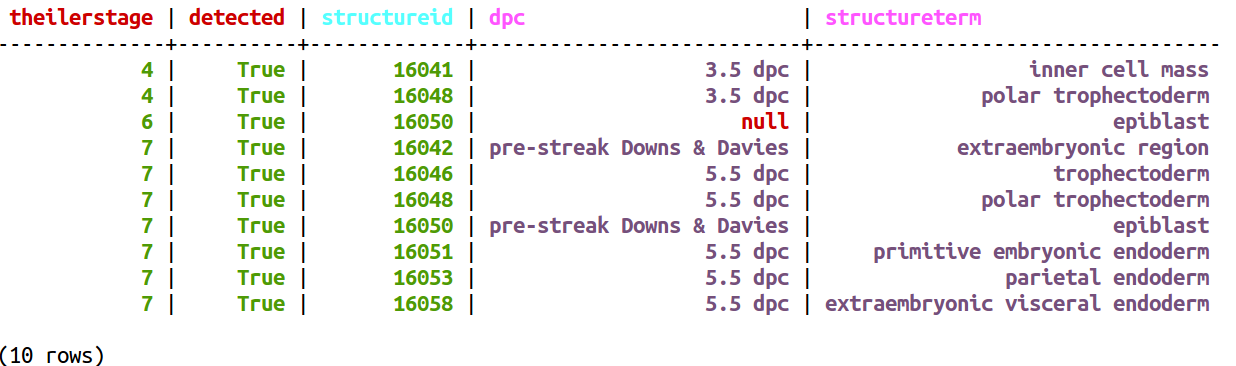
\includegraphics[height=6cm,width=1\linewidth]{images/cassandraquery2}\caption{Cassandra query 2 - All structures between Theiler Stage X and Y}\label{fig:cassandraquery2}\end{center}\end{figure}

\newpage
\subsection*{Query 3 - Where is Gene X expressed?}\label{query3}
The following code snippets represent the queries written for competency question 3.

\begin{itemize}[leftmargin=*]
\item \textbf{MySQL}
\end{itemize}

\begin{lstlisting}[language=SQL, caption=, label=code:mysqlquery3]
SELECT t1.name AS GeneName, t3.term AS StructureTerm, t3.accession AS StructureID
FROM Genes AS t1
INNER JOIN TextAnnotations AS t2
ON t1.id = t2.gene_id
INNER JOIN AnatomyStructures AS t3
ON t2.structure_id = t3.id
WHERE t2.detected = 1
AND t1.name = 'Hoxb13'
GROUP BY 3
ORDER BY 2,3;
\end{lstlisting}

\begin{figure}[H]\begin{center}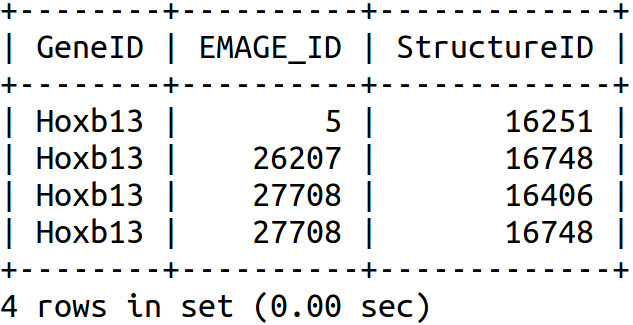
\includegraphics[height=5cm,width=0.7\linewidth]{images/mysqlquery3}\caption{MySQL query 3 - Where is Gene X expressed?}\label{fig:mysqlquery3}\end{center}\end{figure}

\begin{itemize}[leftmargin=*]
\item \textbf{MongoDB}
\end{itemize}

\begin{lstlisting}[language=json, caption=, label=code:mongoquery3]
db.emage.find({ $and: [ { "textannotation.gene.name": "Hoxb13" }, { $or: [ { "textannotation.strength": "detected" }, { "textannotation.strength": "strong" } ] } ] }).pretty();
\end{lstlisting}

\begin{itemize}[leftmargin=*]
\item \textbf{Neo4j}

\end{itemize}\begin{lstlisting}[language=SQL, caption=, label=code:neoquery3]
MATCH (g:Gene)<-[]-(textannotation:TextAnnotation)-[]->(a:AnatomyStructure)
WHERE g.name = 'Hoxb13' AND textannotation.detected = 1
RETURN g.name AS Name, a.accession AS  StructureID, a.term AS Term
ORDER BY a.accession ASC
\end{lstlisting}

\begin{figure}[H]\begin{center}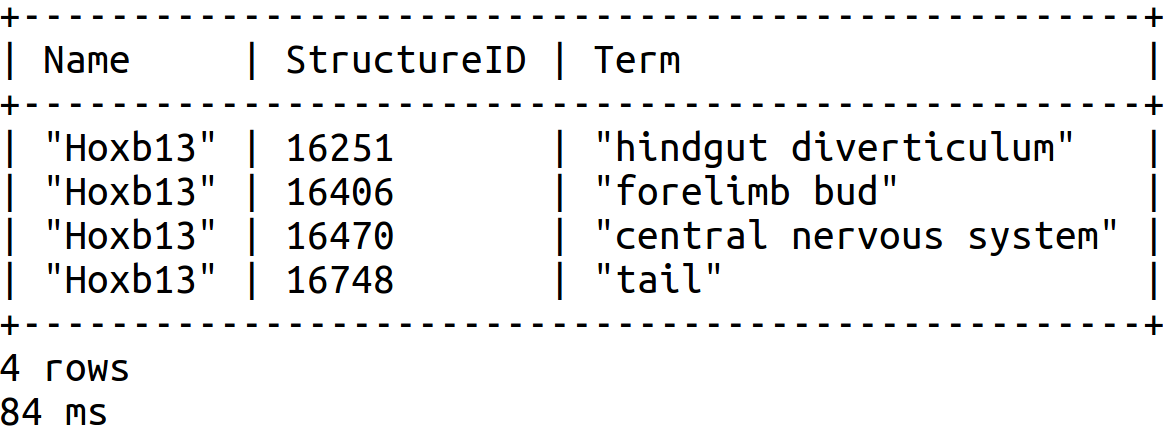
\includegraphics[height=5cm,width=0.6\linewidth]{images/neo4jquery3terminal}\caption{Neo4j query 3 - Where is Gene X expressed?}\label{fig:neo4jquery3terminal}\end{center}\end{figure}

\begin{itemize}[leftmargin=*]
\item \textbf{Cassandra}
\end{itemize}

\begin{lstlisting}[language=SQL, caption=, label=code:cassquery3]
SELECT *
FROM structurebygene3
WHERE genename = 'Hoxb13'
AND detected = true
ALLOW FILTERING;
\end{lstlisting}

\begin{figure}[H]\begin{center}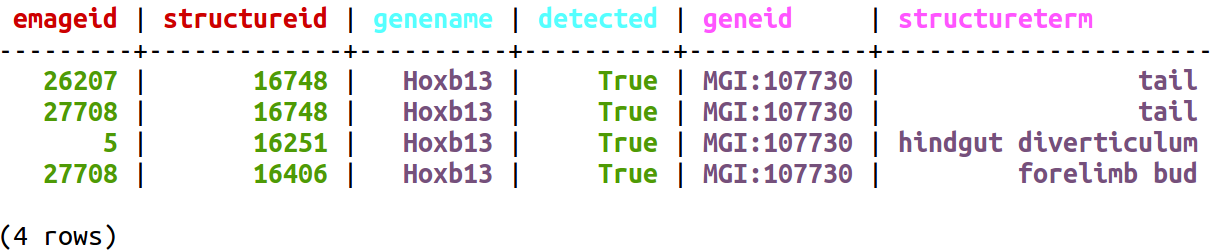
\includegraphics[height=5cm,width=1\linewidth]{images/cassandraquery3}\caption{Cassandra query 3 - Where is Gene X expressed?}\label{fig:cassandraquery3}\end{center}\end{figure}

\newpage
\subsection*{Query 4 - What is expressed in structure X?}\label{query4}
The following code snippets represent the queries written for competency question 4.

\begin{itemize}[leftmargin=*]
\item \textbf{MySQL}
\end{itemize}

\begin{lstlisting}[language=SQL, caption=, label=code:mysqlquery4]
SELECT t1.name AS GeneName, t2.accession AS StructureID, t2.term AS TermName, t4.theilerstage AS TheilerStage, t3.emage_id AS EMAGE_ID
FROM Genes AS t1
INNER JOIN emage.TextAnnotations AS t3
ON t1.id = t3.gene_id
INNER JOIN emage.AnatomyStructures AS t2
ON t3.structure_id = t2.id
INNER JOIN Stages AS t4
ON t2.stage_id = t4.id
INNER JOIN Assays AS t5
ON t3.emage_id = t5.emage_id
WHERE t3.detected = 1
AND t2.accession = 17451
ORDER BY 5;
\end{lstlisting}

\begin{itemize}[leftmargin=*]
\item \textbf{MongoDB}
\end{itemize}

\begin{lstlisting}[language=json, caption=, label=code:mongoquery4]
db.emage.find({ "textannotation.anatomystructure.structureID": 17451 },{},{"_id":1})
\end{lstlisting}

\begin{itemize}[leftmargin=*]
\item \textbf{Neo4j}
\end{itemize}

\begin{lstlisting}[language=SQL, caption=, label=code:neoquery4]
MATCH (stage:Stage)<-[]-(struct:AnatomyStructure)<-[]-(text1:TextAnnotation)-[]->(assay:Assay)
WHERE struct.accession = 17451
RETURN struct.accession AS StructureID, struct.term AS Term,stage.theilerStage AS TheilerStage, assay.emageID AS EMAGEID
ORDER BY assay.emageID ASC
\end{lstlisting}

\begin{itemize}[leftmargin=*]
\item \textbf{Cassandra}
\end{itemize}

\begin{lstlisting}[language=SQL, caption=, label=code:cassquery4]
SELECT *
FROM textannotations1
WHERE structureid = 17451
AND detected = true
ALLOW FILTERING;
\end{lstlisting}

% Please add the following required packages to your document preamble:
% \usepackage{graphicx}
\begin{table}[H]
\centering
\resizebox{\textwidth}{!}{%
\begin{tabular}{|c|c|c|c|c|}
\hline
\textbf{Gene Name} & \textbf{Structure ID} & \textbf{Structure Name} & \textbf{Theiler Stage} & \textbf{EMAGE ID} \\ \hline
Adrbk1 & 17451 & \begin{tabular}[c]{@{}c@{}}interdigital region between\\ forelimb digits 3 and 4\end{tabular} & 20 & 3347 \\ \hline
Lpl & 17451 & \begin{tabular}[c]{@{}c@{}}interdigital region between\\ forelimb digits 3 and 4\end{tabular} & 23 & 7331 \\ \hline
Dll1 & 17451 & \begin{tabular}[c]{@{}c@{}}interdigital region between\\ forelimb digits 3 and 4\end{tabular} & 23 & 7642 \\ \hline
Tshz1 & 17451 & \begin{tabular}[c]{@{}c@{}}interdigital region between\\ forelimb digits 3 and 4\end{tabular} & 23 & 8846 \\ \hline
Trem2 & 17451 & \begin{tabular}[c]{@{}c@{}}interdigital region between\\ forelimb digits 3 and 4\end{tabular} & 23 & 11375 \\ \hline
Klhl5 & 17451 & \begin{tabular}[c]{@{}c@{}}interdigital region between\\ forelimb digits 3 and 4\end{tabular} & 23 & 18331 \\ \hline
\end{tabular}%
}
\caption{My caption}
\label{my-label}
\end{table}

\newpage
\subsection*{Query 5 - Which Genes are stored in structures X and Y?}\label{query5}
The following code snippets represent the queries written for competency question 5.

\begin{itemize}[leftmargin=*]
\item \textbf{MySQL}
\end{itemize}

\begin{lstlisting}[language=SQL, caption=, label=code:mysqlquery5]
SELECT t1.name AS GeneName
FROM Genes AS t1
INNER JOIN TextAnnotations AS t3
ON t1.id = t3.gene_id
INNER JOIN AnatomyStructures AS t2
ON t2.id = t3.structure_id
WHERE t3.detected = 1
AND t2.accession IN (16062, 16069)
GROUP BY 1
HAVING COUNT(DISTINCT t2.accession) > 1;
\end{lstlisting}

\begin{itemize}[leftmargin=*]
\item \textbf{Neo4j}
\end{itemize}

\begin{lstlisting}[language=SQL, caption=, label=code:neoquery5]
MATCH (n:Gene)<-[]-(t:TextAnnotation)-[]->(a:AnatomyStructure)
with count (distinct (a.accession)) as c, t as ta, a as an, n as ge
WHERE ta.detected = 1 and an.accession = 16062 or an.accession = 16069 and c > 1
return distinct ge.name
order by ge.name
\end{lstlisting}

\newpage
\subsection*{Query 6 - Which Genes are most commonly co-expressed?}\label{query6}
The following code snippets represent the queries written for competency question 6.

\begin{itemize}[leftmargin=*]
\item \textbf{MySQL}
\end{itemize}

\begin{lstlisting}[language=SQL, caption=, label=code:mysqlquery6]
SELECT t1.name AS GeneName, COUNT(DISTINCT t2.accession) AS Co_Expressed_Count
FROM Genes AS t1
INNER JOIN TextAnnotations AS t3
ON t1.id = t3.gene_id
INNER JOIN AnatomyStructures AS t2
ON t2.id = t3.structure_id
WHERE t3.detected = 1
GROUP BY 1
HAVING COUNT(DISTINCT t2.accession) > 1
ORDER BY 2 DESC
LIMIT 5;
\end{lstlisting}

\begin{figure}[H]\begin{center}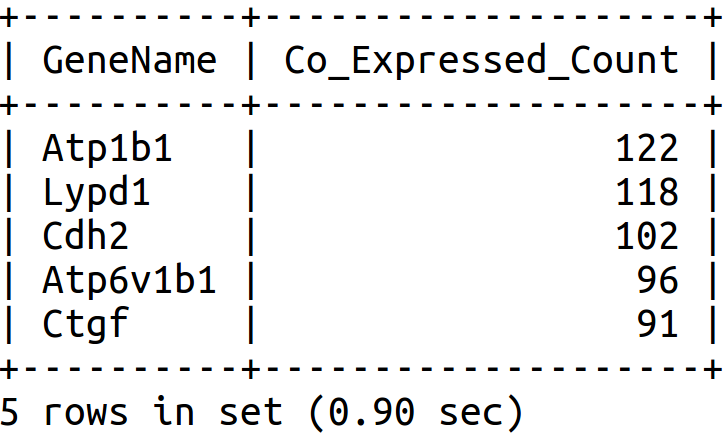
\includegraphics[height=5cm,width=0.7\linewidth]{images/mysqlquery6}\caption{MySQL query 6 - Which Genes are most commonly co-expressed?}\label{fig:mysqlquery6}\end{center}\end{figure}

\newpage
\subsection*{Query 7 - Calculate transitive closure}\label{query7}
The following code snippets represent the queries written for competency question 7.

\begin{itemize}[leftmargin=*]
\item \textbf{MySQL}
\end{itemize}

\begin{lstlisting}[language=SQL, caption=, label=code:mysqlquery71]
SELECT DISTINCT tmp.term, t1.parent_term AS lev1, t2.parent_term AS lev2, t3.parent_term AS lev3, t4.parent_term AS lev4
FROM Closure AS t1
INNER JOIN AnatomyStructures AS tmp
ON t1.child_id = tmp.accession
LEFT JOIN Closure AS t2 ON t2.child_id = t1.parent_id
LEFT JOIN Closure AS t3 ON t3.child_id = t2.parent_id
LEFT JOIN Closure AS t4 ON t4.child_id = t3.parent_id
WHERE tmp.accession = 16201
\end{lstlisting}
\begin{figure}[H]\begin{center}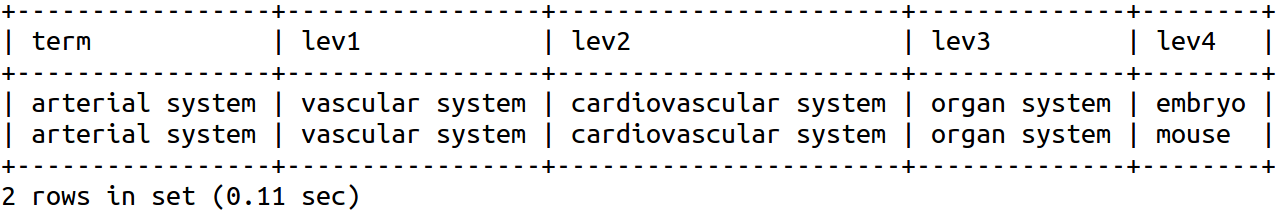
\includegraphics[height=4cm,width=1\linewidth]{images/mysqlquery71}\caption{MySQL query 7 - Calculate transitive closure}\label{fig:mysqlquery7}\end{center}\end{figure}

\begin{lstlisting}[language=SQL, caption=, label=code:mysqlquery72]
SELECT distinct tmp.term, t1.parent_term AS lev1, t2.parent_term as lev2, t3.parent_term as lev3, t4.parent_term as lev4, t5.parent_term as lev5, t6.parent_term as lev6
FROM Closure AS t1
INNER JOIN AnatomyStructures as tmp
ON t1.child_id = tmp.accession
LEFT JOIN Closure AS t2 ON t2.child_id = t1.parent_id
LEFT JOIN Closure AS t3 ON t3.child_id = t2.parent_id
LEFT JOIN Closure AS t4 ON t4.child_id = t3.parent_id
LEFT JOIN Closure AS t5 ON t5.child_id = t4.parent_id
LEFT JOIN Closure AS t6 ON t6.child_id = t5.parent_id
WHERE tmp.accession = 16205;
\end{lstlisting}
\begin{figure}[H]\begin{center}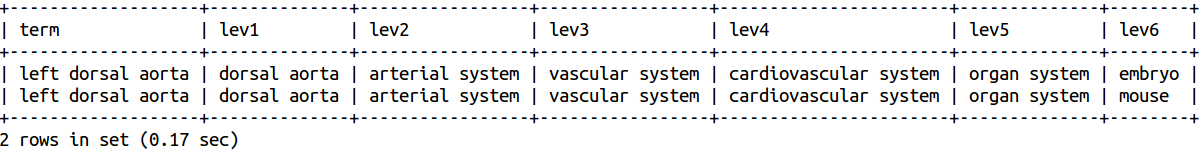
\includegraphics[height=4cm,width=1\linewidth]{images/mysqlquery72}\caption{MySQL query 7 - Calculate transitive closure}\label{fig:mysqlquery7}\end{center}\end{figure}


\section{System Evaluation}\label{queryevaluation}